\section{Qualitätsmessung der Kompression}
Um die Datenmenge der Feldlinien zu verringern werden verlustbehaftete Kompressionsverfahren angewendet. Trotz des Dateverlustes sollen die dekomprimierten Linien möglichst ihren Originalen ähneln. Kleine Abweichungen werden von den Sonnenforschern toleriert. Ihnen ist wichtig, dass vorallem die Form der Kurve möglichst erhalten bleibt. Grosse Abweichungen, die selten eintreten, können aber das Aussehen einer Kurve grundlegend verändern.\\
[\baselineskip]
Zusammen mit den Sonnenforschern wurden zwei Fehlermasse bestimmt: Der absolute maximale Fehler und die Standardabweichung von der komprimierten Linie zum Original. 
formel der Standardabweichung, grosse Abweichungen werden stärker gewichtet.\\
Der absolute maximale Fehler wird noch als Absicherung gemessen. In den meisten Fällen wird die Kompression mit der tieferen Standardabweichung auch den kleineren maximalen Fehler haben. Da aber die Messung über ein paar hunderttausend Punkte durchgeführt wird, ist das Gegenteil denkbar. Eine gute Kompression muss es einen minimalen absoluten Fehler haben und eine minimale Standardabweichung bei minimalem Platzbedarf.\\
[\baselineskip]
Eine feste Grenze für die Genauigkeit ist leider nicht objektiv festzulegen. Auch wenn eine Grenze gefunden wird, kann diese sich in der Zeit verändern. Im Fall der Feldlinien ist die Internetverbindung der Flaschenhals. Es kann sein, dass in Zukunft mehr Präzision bei mehr Platzbedarf verlangt wird. Deshalb werden die Verfahren, wenn möglich, mit unterschiedlichen Qualitätsstufen getestet und verglichen.
\begin{figure}[!htbp]
	\center
	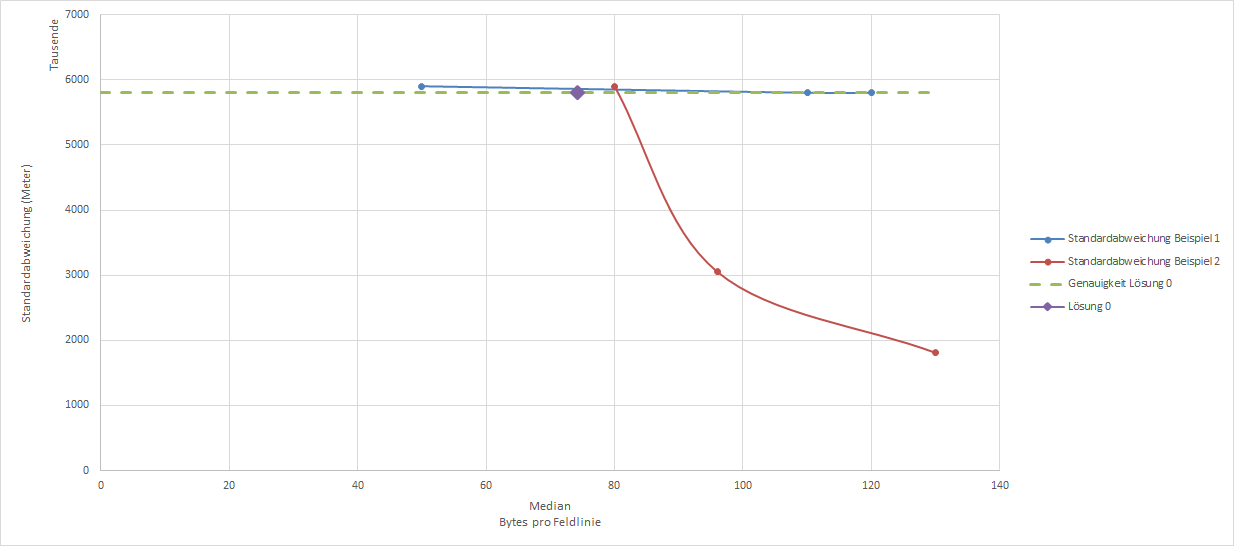
\includegraphics[width=0.8\textwidth,height=6cm,keepaspectratio]{./pictures/testsetup/Beispielgraph.png}
	\caption{Beispiel eines Vergleichsdiagramms. Auf der X-Achse ist die durchschnittliche Anzahl Bytes pro Feldlinie dargestellt. Die Y-Achse zeigt die Standardabweichung in Meter an. Die rote und blaue Kurven sind Beispieldaten}
	\label{testsetup:beispielgraph}
\end{figure} 
Die Abbildung \ref{testsetup:beispielgraph} zeigt ein Vergleichsiagramm, welches im Abschnitt \ref{resultate} verwendet wird. Es werden die Standardabweichungen von zwei Beispielansätzen mit der Lösung 0 verglichen. Der Violette Punkt stellt die Lösung 0 dar, der grüne Strich ist eine hilfslinie und zeigt die Genauigkeit der Lösung 0 an. Damit eine Kompression besser ist, muss sie links und unterhalb des Violetten Punktes hingelangen.

\subsection{Auswahl und Erhebung der Testdaten}
Die Testdaten sollen zu einem alle Randfälle abdecken, als auch durchschnittliche Fälle enthalten. Aus diesem Grund wurden insgesamt zehn Datensätze ausgewählt: Vier Datensätze mit hoher Sonnenaktivität, zwei mit wenig und vier zufällig. Für die vier Datensätzen mit hoher Aktivität wurde in den Jahren 2014 und 2013 nach den grössten Solare Flares gesucht. Für die Datensätze mit wenig Aktivität wurde das Gegenteil gemacht, nach Zeiträumen mit möglichst kleinen Solar Flares gesucht.\\
Die feldlinien werden aber nur alle sechs Stunden berechnet und Solar Flares sind sehr spontane Ereignisse. Auch eine grosse Flare kann während den sechs Stunden angefangen und wieder aufgehört haben. Für die grossen Solar Flares wurde deshalb beachtet, dass die Datensätze vor dem Ereignis verwendet wurden. Grosse Solar Flares entladen das Feld, vor dem Ereignis ist das Magnetfeld komplexer.\\
[\baselineskip]
Wie im Abschnitt \ref{konzept:ist-komprimierung} beschrieben, führt der IDL-Code schon eine Quantisierung durch. Diese wurde entfern und  deshalb wurde der IDL Code angepasst. Die Quantisierung wurde für die Testdaten entfernt. Die Punkte werden nun mit 32 Bit Floating-Point Genauigkeit gespeichert.

\subsection{Aublauf des Tests und Messung des Fehlers}
Float daten werden geladen. Daten kopiert und Kompression/Dekompression durchgeführt für alle Testdaten. Die kopierten Daten wissen aber noch, welches ihr Originalpunkt ist.
Zwei Mengen, Originalpunkte $O$, dekomprimierte Punkte $D$. Es gibt immer gleich viele oder mehr Originalpunkte wie dekomprimierte Punkte. Die Fehlerberechnung muss der allgemeine Fall und die Randbehandlung unterschieden werden.

\subsubsection{Allgemeiner Fall}
\begin{figure}[!htbp]
	\center
	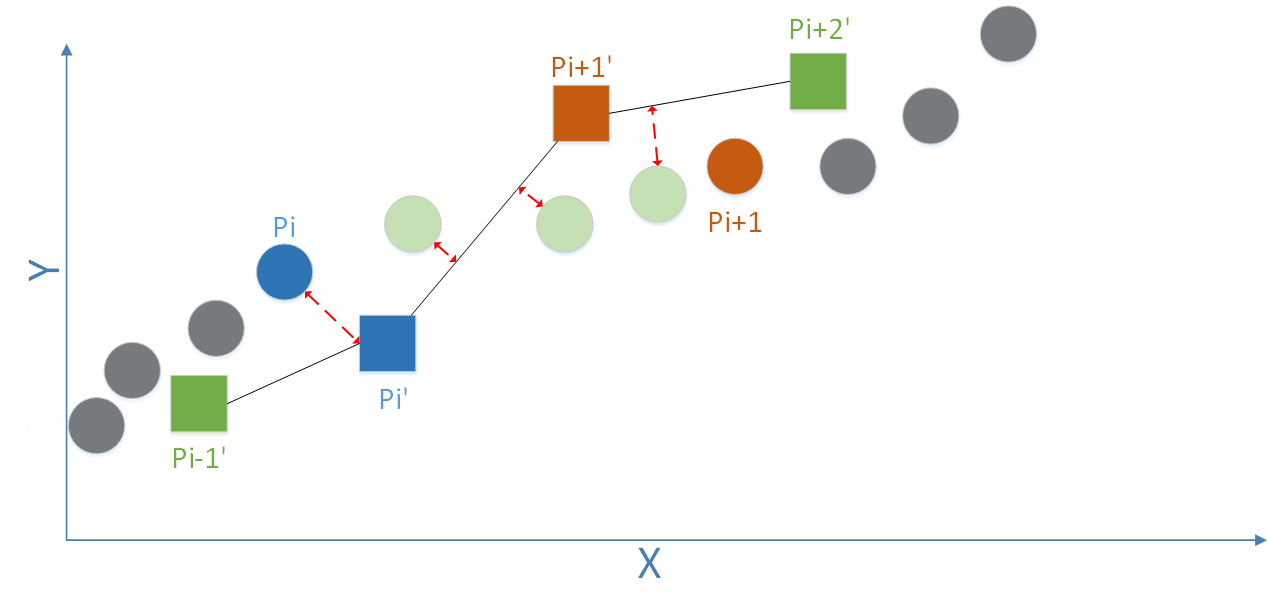
\includegraphics[width=0.8\textwidth,height=6cm,keepaspectratio]{./pictures/testsetup/errorcalc.png}
	\caption{Darstellung der Fehlerberechnung. Die Punkte sind die Originaldaten, die Quadrate sind die Punkte nach der Kompression.}
	\label{testsetup:ablauf:fehlerberechnung:diagramm}
\end{figure} 
Die Berechnung ist Dargestellt im Diagramm \ref{testsetup:ablauf:fehlerberechnung:diagramm}. Für jeden Punkt $p1'$ aus $D$, nehme $p1'$ und den folgenden Punkt und $p2'$. Ziehe eine Strecke $s$ durch $p1'$ und $p2'$. Suche von $p1'$ den Originalpunkt $p1$ aus $O$ und rechne den Abstand aus zur Strecke $s$. Führe das für alle folgenden Originalpunkte durch, bis $p2$ erreicht wurde. Der Abstand $s$ zu $p2$ wird nicht mehr berechnet.\\
[\baselineskip]
\textbf{Abstandsberechnung eines Punktes zu einer Strecke}\\
Gegeben: Stecke $s$ mit Eckpunkten $A$ und $B$ und Punkt $P$.\\
Gesucht: Kürzeste Distanz zwischen $s$ und $P$\\
[\baselineskip]
Zuerst wird überprüft, ob eine Senkrechte durch $P$ überhaupt auf der Strecke $s$ zu liegen kommt. Das ist der Fall, wenn die Strecke $AP$ auf die Strecke $s$ projizierbar ist.



\subsubsection{Randbehandlung}


\subsubsection{Berechnung der Standardabweichung}
